\documentclass[12pt,halfparskip]{scrreprt}

\usepackage{pystructure}

\usepackage{svn} % For handling of SVN keywords
\SVN $LastChangedDate$

\begin{document}

\begin{titlepage}

\pagenumbering{alph}
\thispagestyle{empty}

\begin{center}

\begin{figure}[h]
 \centering
 \vspace{0,5cm}
 
\includegraphics[width=\textwidth]{img/hsr_logo}
\end{figure}

\vspace{1cm}
{\Large \bfseries HSR -- University of Applied Sciences Rapperswil}

\vspace{0,5cm}
{\Large \bfseries Institute for Software}

\vspace{2cm}
{\Huge \bfseries PyStructure -- Automated Structure and Dependency Analysis of Python Code}

% { TOOD delete me 
{\Large \bfseries DRAFT VERSION}
%}

\vspace{2cm}

{\Large \bfseries Bachelor Thesis: Spring 2008}

\vspace{0,5cm}
\SVNDate


\vspace{1cm}
Reto Schüttel \\ \url{reto@schuettel.ch}

\vspace{0,5cm}
Robin Stocker \\ \url{robin@nibor.org}

\vspace{0,5cm}
Supervised by Prof. Peter Sommerlad

% FIXME external partner

\vspace{1cm}
\url{http://pystructure.ifs.hsr.ch/}

\end{center}
\end{titlepage}


\pagenumbering{roman}
\pagestyle{plain}

%%%%%%%%%%%%%%%%%%%%%%%%%%%%%%%%%%%%%%%%%%%%%%%%%%%%%%%%%%%%%%%%%%%%%%%
\chapter*{Abstract}


%%%%%%%%%%%%%%%%%%%%%%%%%%%%%%%%%%%%%%%%%%%%%%%%%%%%%%%%%%%%%%%%%%%%%%%
\chapter*{Management Summary}

\section*{Motivation}

\section*{Goal}

\section*{Results}

\section*{Outlook}


\newpage

\tableofcontents

\newpage
\pagenumbering{arabic}
\pagestyle{scrheadings}

%%%%%%%%%%%%%%%%%%%%%%%%%%%%%%%%%%%%%%%%%%%%%%%%%%%%%%%%%%%%%%%%%%%%%%%
\chapter{Introduction}

\section{Structural Analysis}

Structural Analysis

%%%%%%%%%%%%%%%%%%%%%%%%%%%%%%%%%%%%%%%%%%%%%%%%%%%%%%%%%%%%%%%%%%%%%%%
\chapter{Type Inference}

\section{Introduction}

\subsection{Idea – Why inferring types?}

Before any meaningful structure analysis of a program is possible the individual components have to be identified and analysed. To know what dependencies a component (e.g. a class) has, it first has to be determined what kind of other components are being used. For example if the GUI class calls a method of a class in the business logic we clearly have a dependency between these two components. It becomes obvious that knowing the type of a given expression, in this example the method call, is imperative for any meaningful structural analysis.

This leads to the question, how can the type of a given expression be determined? In Java this question would be very simple, the definition always states the type.\footnote{In the example \code{boolean isOdd(int i)}, method \code{isOdd} has a parameter \code{i} with the type \type{int} and returns a \type{boolean}.} In Python the types aren't specified at all, they are only known at runtime by the interpreter. To still be able to determine them, a heuristic has to be used which infers the types by looking at the context and finding answers to questions like ``Where was the variable defined?'' and ``Who called that function?''. This heuristic is usually called type inferencer (TI).

\subsection{Goal}

So, developing a type inferencer was a central goal of the project. To be useful for structural analysis, it should be able to resolve the type of the following expressions:

\begin{itemize}
	\item Local \& global variables
	\item Arguments
	\item Attributes
	\item Return values of functions \& methods
\end{itemize}

Of course the type inferencer should take the application as a whole into account and develop a best guess what the given expression's type could be. For example in the case of a method argument, the type inferencer should look for all places where the particular method is called and what argument type was used.

The type inferencer should also be able to handle the case where more than one type is possible for a single expression, a simple example\footnote{The ternary operator is a bit different in Python than in other languages, the example means: \code{vehicle = (input == "car") ? Car() : Plane()}} would be:

\begin{lstlisting}
vehicle = Car() if input == "car" else Plane()
\end{lstlisting}

In this case the type inferencer has to realise that \code{vehicle} can be \type{Car} or \type{Plane}.

{Concept}

(Goal engine, why \& how) \\
(link to other possible solutions)
Correctness \& Usefulness


\section{Process Overview}

The type inferencer is divided into three main process stages:

\begin{itemize}
	\item Parser – Parses the source code and generates an abstract syntax tree (AST)
	\item Definition Visitor – Builds a model of the program
	\item Type Inferencer – Evaluates the type of an expression
\end{itemize}

\begin{figure}[h!]
 \centering
 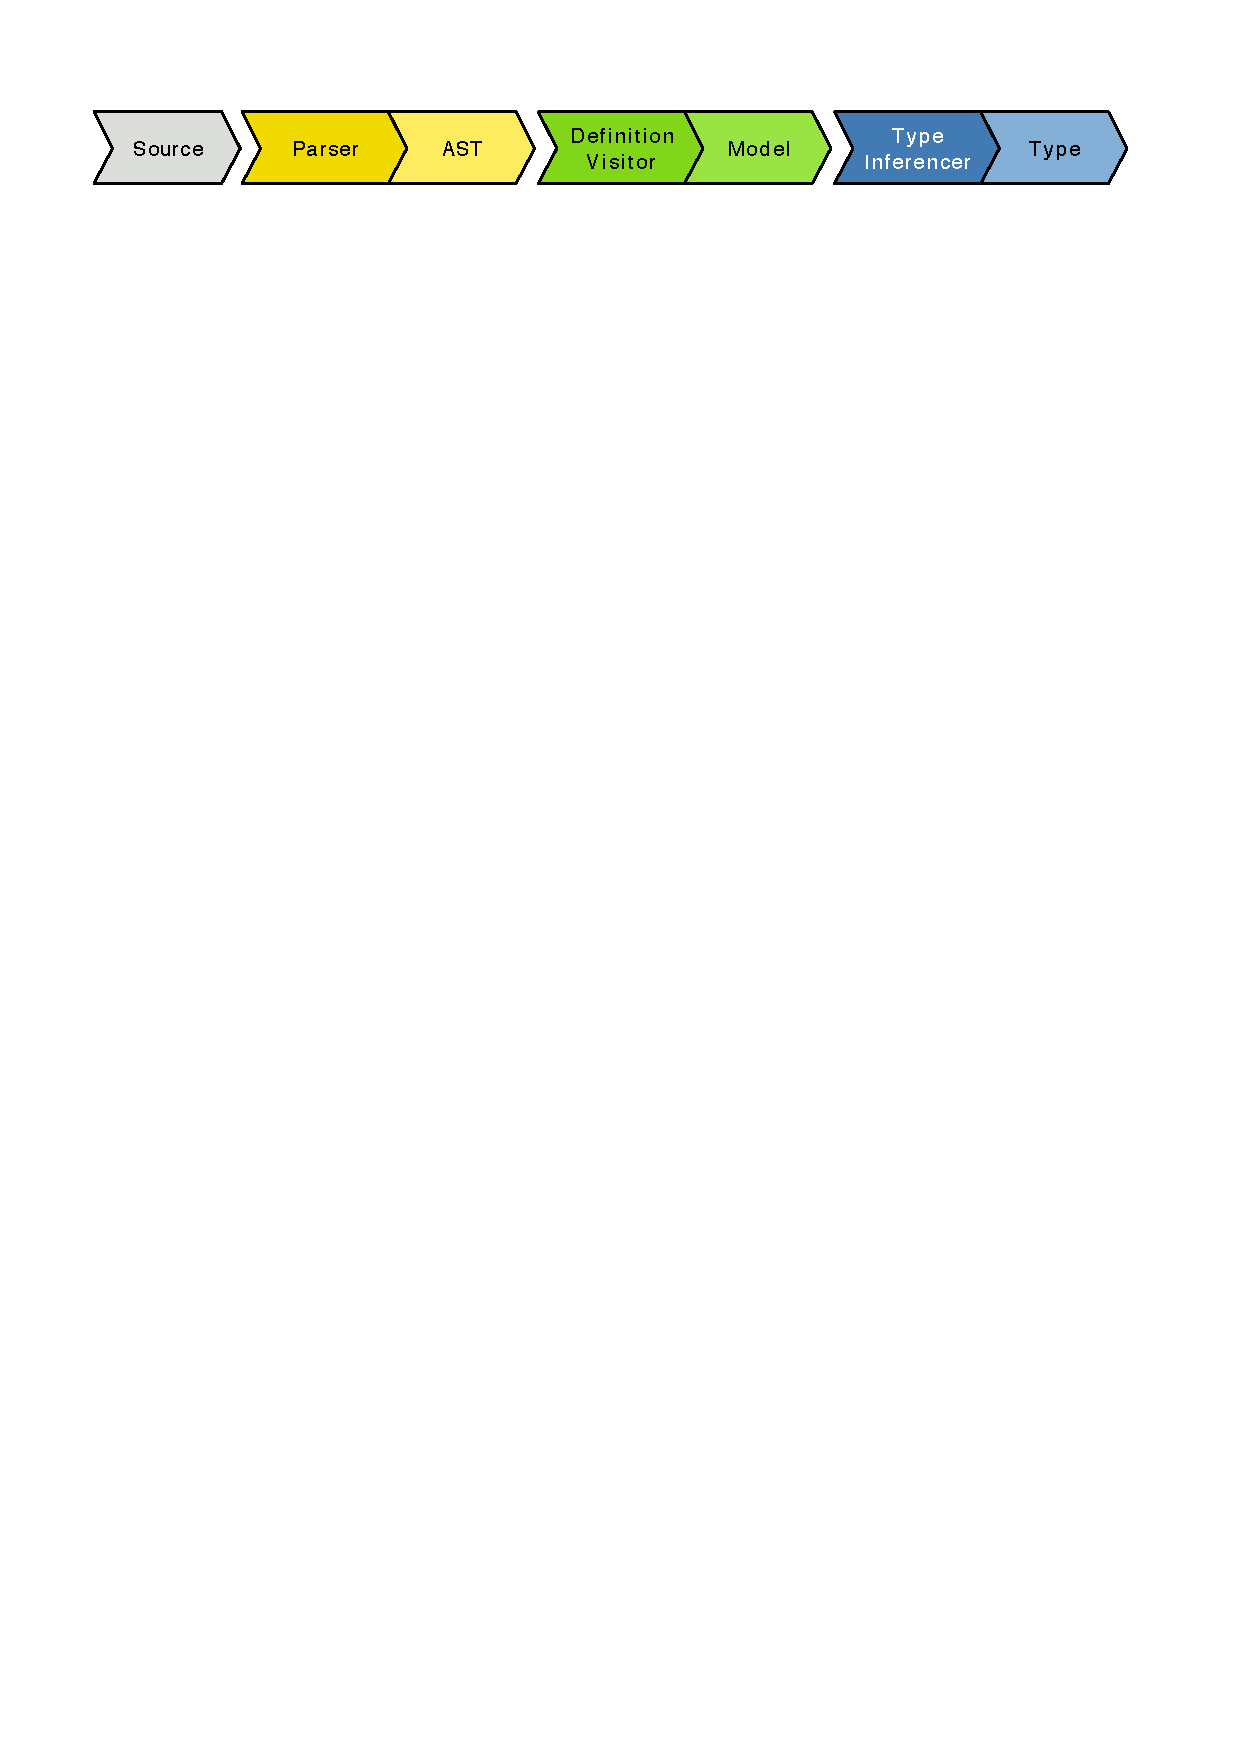
\includegraphics[width=1 \textwidth]{process_overview}
 \label{fig:process_overview}
\end{figure}

The first two steps, the parsing of the source code and the generation of the model, lay the foundation for the type inferencer. They do a static analysis of the whole project and are independent of what expressions should be evaluated. As long as the underlying source code doesn't change these preparations can be reused for any number of type inferencer evaluations.


\section{Parsing the Source Code}

Before any analysis can be done on the application its source code has to be brought into a form which is easier to process for programs. It's quite common to express an application's source code as a tree, where an interior node represents a programming language construct and the children of that node represent meaningful components of the construct. For example the simple code \code{foo("bar")} is a call node with the parameter as a string node attached to it. This node structure is usually called abstract syntax tree (AST).

\begin{lstlisting}
Call
|   func = Name("foo"),
|   args = 
|   |   Str("bar")
\end{lstlisting}

Instead of writing a new parser, PyStructure uses a modified version of the Jython\footnote{Jython is a Python implementation for the JVM written in Java.} parser. The modifications were done by the PyDev\footnote{PyDev is an IDE for Python developers based on Eclipse and written in Java.} project to be able to interpret Python 2.5 source code, the normal Jython parser can only parse source code written for Python 2.2. In the long term it would be advantageous to use the unmodified Jython parser, but before 2.5 syntax is supported this is not really an option.

%{ Robin: ist Abschnitt wirklich wichtig? 
It should be noted that the parser does not do that much beside converting the source code into a tree representation. It for example doesn't do any transformation of expressions which can be written in different ways. For example the expression \code{a + b} is handled by the Python interpreter as \code{a.__add__(b)}, but the parser still interprets the code as \node{BinOp(a, b, op=Add)} and therefore distinguishes it from literally calling the \code{__add__} method, which would be \node{Call(a.__add__, args=b)}. 
%}


\section{Creating the Model}

% { rstocker: bisschen korrigiert, gefällt mir aber immer noch ned super. 

The representation of a program provided by the AST is very basic and working directly with it is quite cumbersome. 
One drawback of the AST is that it's just a \emph{syntactical} representation of the source code and doesn't include any semantic information. For example, in the following code, the AST doesn't know that the two uses of \id{foo} are related:

\begin{lstlisting}
foo = "Hello"
print foo
\end{lstlisting}

Therefore PyStructure uses a second stage in which it processes the AST further and does some static analysis which then can be used by the type inferencer.

% }

\subsection{Creating the Structure}

The first step of building the model is to extract the structural elements that make up a program, like modules, classes, methods and functions. These also represent scopes for variables.

Creating this initial structure is done by the \class{StructureDefinitionVisitor}. It is a simple visitor which just visits class and function definitions.\footnote{Method definitions are the same as function definitions in the AST, and in the Python language itself} Then it creates \class{Class}, \class{Function} and \class{Method} objects. These objects wrap the AST nodes and also provide additional functionality, for example \class{Class} knows which methods it includes. They also know which child structures are within them so that visiting them later is easier.

\subsection{Connecting Definitions and Uses}

Now we have the elements of the model, but there's not yet very much information provided by it. As described in the example with the \id{foo} variable, knowing which variable definitions and uses are related would be very useful. This is part of what the \class{DefinitionVisitor} does and is called flow analysis.

Flow analysis is an important part of type inference. In Python, it is possible that a variable is assigned multiple times with different types. This doesn't matter if the values are assigned sequentially and without any \code{if} blocks:

\begin{lstlisting}[numbers=left]
var = 42
print var

var = "Hi"
print var
\end{lstlisting}

The flow analysis deals with these two elements:

\begin{description}
	\item[Definition] Binding of a value to a name, e.g. an assignment or a \code{for} loop variable.
	\item[Use] Reference of a name, e.g. a variable name.
\end{description}

In the example, both occurrences of \id{var} on line 1 and 4 are definitions and those on lines 2 and 5 are uses. The two definitions are made unconditionally, which means the two uses each belong to the definition right before them. So, when the types are inferred, the first \id{var} is \type{int} and the second is \type{str}.

If an analyser doesn't actually respect the flow of the variables and just takes all assignments to the same name as belonging to the same variable, it is called flow-insensitive. In the example this would mean that both uses would be connected to both definitions.

% todo: does this sound redundant?

PyStructure is flow-sensitive, which means it is as precise as possible when there's more than one assignment of a variable in the same scope. The advantage is that it results in better precision for inferring types and it is also a very useful feature to have for the use case of an IDE, where it helps with certain refactorings.

It should be noted that at this point, no types are involved, it just deals with definitions and uses of names. In the following examples, types are only used to illustrate how the flow analyser should connect definitions and uses.

\subsubsection{Branches}

When conditional assignments are involved, it is more difficult to clearly say which type a variable is of:

\begin{lstlisting}
if sometimes_true():
    x = 42
    print x
else:
    x = 3.14
    print x
print x
\end{lstlisting}

At the first \code{print} statement, \id{x} is of type \type{int}. At the second, it is of type \type{float}, because of the assignment above it. At the \code{print} statement after the if/else block, it is of type \type{int|float}, because which branch is executed is only determined at runtime. Therefore the engine has to say that both types are possible. 

\subsubsection{Scopes}

If a variable from an outer scope is read, it isn't possible to specifically determine its type, because that depends on where the variable is assigned:

\begin{lstlisting}
def func():
    print g

g = 1
func()

g = 3.14
func()
\end{lstlisting}

The two calls of \id{func} will print values of different types, because the outer variable \id{g} is accessed after it has been assigned another value. In the function itself, it's not possible to say if the type is \type{int} or \type{float}, because both are possible, so the resulting type is \type{int|float}.

\subsubsection{Global Variables}

Global variables complicate the flow analysis, because they can be assigned from anywhere:

\begin{lstlisting}
g = 1

def func():
    global g
    g = 3.14

print g
func()
print g
\end{lstlisting}

Between the two \id{print} statements, the variable \id{g} was assigned another value from within \id{func}. Therefore, the variable \id{g} in the global scope is of type \type{int|float}.

\subsubsection{Implementation}

Flow analysis as shown above is primarily implemented in the \class{DefinitionVisitor}. It visits the AST and registers \emph{definitions} and \emph{uses} of names (variables, methods, classes). Each use can have multiple possible definitions associated with it, and each definitions can have multiple uses. In other words, they have a many-to-many relationship.

To resolve the definition of a name, it uses a structure of nested blocks and scopes. Scopes are introduced by \code{class} and \code{def} statements, and there's also a scope for the module the code is in. Blocks correspond to lines of code which are usually grouped by indentation\footnote{Python actually makes indentation even mandatory and therefore doesn't need block delimiters like curly braces or end statements.}. Scopes are blocks too, just with special semantics. The following example is used to explain the algorithm:

\begin{lstlisting}[numbers=left]
x = "unrelated"
print x

def func():
    x = 1
    if random():
        y = 42
        print x
    else:
        y = 3.14
        print y
    print y

func()
\end{lstlisting}

The first line defines a variable with the name \id{x}, the second is a use of this definition.

On line 4, there's a function definition with the name \id{func}. It introduces a scope for the function. Because in the scope of the function, variables from the whole outer scope could be used, the visiting of the function body is deferred to later.

Line 14 is a name use of \id{func}. That it is a function call doesn't matter for the \class{DefinitionVisitor}.

The visitor now visits the body of the function. The scope of the function is created, with the module scope as the parent scope. At line 5, there's a definition of the name \id{x}.

At line 7, a block starts for the if clause and there's a definition for \id{y}. Line 8 uses the \id{x} variable. To find the corresponding definition(s), the enclosing block is searched for the current definition of \id{x}. The search continues to the next parent block if it isn't found. So the definition from line 5 is found and the use associated with it.

At line 10, the else clause begins. There's another definition of \id{y} here. Line 11 uses \id{y} and its definition is found directly in the block.

On line 12, the two blocks of the if have ended. The definitions of both blocks are now set as the current definitions of \id{y}, they are said to flow out from the block. So the use on this line may refer to both the definitions in the if/else block and the use is created accordingly.

No definitions flow from the scope, so the visitor has done its work and can return the results, the name uses and definitions.

\subsection{Limits of the Model}

There are things which are not represented in the model because it is built without using type inference. Some of these things are:

\begin{itemize}
	\item Which data attributes a class has isn't known, because they are not declared anywhere, they are just assigned as needed.
	\item The class hierarchy isn't known in advance, because the specification of the base class is just an expression and could be the result of a function call or an imported class.
	\item What exactly is being imported by an import statement.
	% rschuett: Hast du noch mehr Ideen?
\end{itemize}


\section{Inferring Types}

Now, after all the source has been parsed an a generalised model of the program has been build the actual analysing can begin. 

In the first part of this section the actual evaluation process is explained and the second part describes the underlying goal engine which is responsible for organising the different goals during the evaluation.

\subsection{Evaluation}

Summarised, the evaluation works as follows: The user of the library picks an expression somewhere in the code and then creates an ``expression type goal'' for this expression. This goal, called root goal, is then fed into the goal engine which starts to process it. Every goal has to be processed by one of the evaluator. Which evaluator has to be used is determined by the evaluator factory according to the goal's type and other criteria. The particular evaluator then gets initialised and processes the goal. The evaluator can (and usually will) create subgoals which are then processed as well. As the goals are being successfully finished their result are reported back to their parent goal. As soon as the root goal finishes, the result is returned to the user.

\subsubsection{Picking a root goal}

As a first step the user of the type inferencer has to create a root goal which describes the actual main goal. Usually this goal is an \class{ExpressionTypeGoal} which instructs the goal engine to determine the type of a given expression (hence the name). The expression in question can be any expression from the AST. They can for example be found by using a visitor like the \class{ExpressionAtLineVisitor} or by iterating over all expressions (like the type spider does \todo{reference to the Spider}).

\subsubsection{Select evaluator for goal}

When the root goal is created it has to be fed into the goal engine. Every goal has to be processed by one of the available evaluators. Which one has to be used is determined by the so-called evaluator factory (class \class{PythonEvaluatorFactory}) which returns the appropriate evaluator depending on the kind of goal and possibly other criteria.

For example in the case of an expression type goal the evaluator factory also considers the type of the associated expression. For example if the expression is a method call the goal gets delegated to the \class{CallTypeEvaluator}, an attribute expression is processed by the \class{AttributeTypeEvaluator} and so on.\todo{Should we a provide a list of these mappings somewhere}

\subsubsection{Evaluator}

Now the actual work begins, the evaluator gets initialised with the goal as a parameter. As a first step the eveluator's \id{init()} method is called. The evaluator then has a first chance to do it's job. If necessary (and it often is) the evaluator can create subgoals and return them. The evaluator's goal is not considered finished as long as there are any remaining subgoals. Every time a subgoal is finished the evaluator's \id{subgoalDone(subgoal)} method is called. Here again the evaluator has the chance to create some subgoals.

From the goal engine's perspective there's no difference between subgoals and root goals, they are handled equally. But of course as soon as the root goal is finished the evaluator returns the found result to the user.

\subsection{Examples}

\todo{here we describe the actual function of the TI by some examples}

Goal Engine \\
 (description of the goal engine)\\
 (advantages/disadvantages)\\
Evaluation\\
 (goals \& evaluators explained)\\
 (examples)


\subsection{Goal Engine}

The goal engine is the central piece which does all the coordination between evaluators and goals. It basically has a working queue of goal nodes, which is the combination of a goal and the evaluator which was created to evaluate the goal. The algorithm works like in this simplified pseudocode:

\begin{lstlisting}
def evaluate_goal(root_goal):
    queue = []
    add_goal(queue, root_goal)

    while len(queue) != 0:
        goal_node = queue.pop()

        if goal_node.is_new():
            subgoals = goal_node.init()
            add_goals(queue, subgoals)

        if goal_node.are_all_subgoals_done():
            goal_node.finish()
            for parent in goal_node.parents:
                subgoals = parent.subgoal_done(goal_node)
                add_goals(queue, subgoals)
        else:
            queue.add(goal_node)
\end{lstlisting}

\todo{describe some goal engine behaviors like, cyclic recursion, caching, crazy ordering and so on}

\section{Challenges/Problems}

In this section, some of the difficult parts of developing a type inference system for Python are described in more detail. Each problem is illustrated with examples and shows the solution which was implemented in PyStructure is explained.

\subsection{Recursion}

\todo{describe recursion}

\subsection{Contexts}

The return type of a function or method may depend on the types of its arguments. An inferencer can be more precise if it treats calls with different arguments differently. The following example shows such a function used with two different arguments:

\begin{lstlisting}
def add_one(value):
    return value + 1

a = add_one(41)
b = add_one(1.5)
\end{lstlisting}

Without separating these two uses, the type inferencer would answer that the type of both \id{a} and \id{b} is \type{int|float}. But a more precise answer would be that \id{a} is \type{int} and \id{b} is \type{float}.

% TODO: Solution, InstanceContext

\subsection{Container Element Types}

When using container types like \id{list} or \id{dict}, each instance of such a type should be treated differently regarding the type of the contained elements. Considering this example:

\begin{lstlisting}
list_a = list()
list_b = list()

list_a.append(42)
list_b.append("x")

a = list_a[0]
b = list_b[0]
\end{lstlisting}

What should the types of the two variables at the end be? Of course it should be \type{int} for \id{a} and \type{str} for \id{b}. But with a type inferencer not aware of different instances, the result is actually \type{int|str} for both variables. Why is that? Let's look at another example of the same problem where we can see what the implementation of the container class is:

\begin{lstlisting}
class Container(object):
    def set(self, element):
        self.element = element

    def get(self):
        return self.element

c1 = Container()
c2 = Container()

c1.set(42)
c2.set("x")

a = c1.get()
b = c2.get()
\end{lstlisting}

The types for \id{a} and \id{b} are the same as in the example with the lists. The problem becomes clear when looking at the evaluation for the type of \id{a} (the finding of references was omitted for brevity):

\begin{enumerate}
	\item[1.] What is the return type of \code{c1.get()}?
	\begin{enumerate}
		\item[2.] What is the type of \code{c1}?
		\item[] $\rightarrow$ The type is \type{Container}.
		\item[3.] What is the type of \code{c1.get}?
		\item[] $\rightarrow$ It is the \id{get} method in the \id{Container} class.
		\item[4.] What is the type of \code{self.element} in the \id{get} method?
		\begin{enumerate}
			\item [5.] What is the type of the \code{element} argument of the \code{Container.set} method?
			\item [] $\rightarrow$ The type is \type{int|str} (from the two \code{set} calls).
		\end{enumerate}
	\end{enumerate}
	\item [] $\rightarrow$ The type is \type{int|str}.
\end{enumerate}

So the problem is that the inferencer treats the \id{Container} class as if every instance had the same type of the \id{self.element} attribute. It doesn't differentiate between instances, only between classes.

... \cite{ddp}

% TODO: Solution (ClassType with constructorCall, InstanceContext), references (Lex Spoon, context from other paper)

\subsection{Inheritance}

\todo{Write me}

Inheritance\\
 (C3 MRO)

\subsection{Built-in Types and Functions}

What would a language be without its built-in types, like \type{int}, \type{str} or \type{list} for Python? Nothing, because all our own code is based on these data structures provided by the language. Similarly, what would a type inference system be without support for these built-in types? Not very usable, as shown in the following example:

\begin{lstlisting}
foos = list()
foos.append(Foo(1))
foos.append(Foo(2))
for element in foos:
    print element
\end{lstlisting}

If the type inferencer had no knowledge of how the \id{list} type works, it wouldn't be able to determine the type of \id{element}. For example, it doesn't know what \id{append} does, because it's not specified anywhere.

\subsubsection{Specifying the Behaviour}

Two of the possible solutions for making the inferencer aware of built-in types are:

\begin{enumerate}
	\item Add special evaluators for evaluating built-in types and implement the rules in Java code.
	\item Create prototype implementations in Python code, which type-wise behave like the original Python implementation..
\end{enumerate}

% rstocker, hab jetzt die liste oben anders gemacht, dafür ist jetzt der satz unten redundant.

The second solution was chosen as it is both cleaner and easier to implement. A prototype implementation works by defining the functions and methods so that they return the same type as the original ones. The following extract from the implementation of the \id{list} type illustrates the concept:

\begin{lstlisting}
class list(object):

    def append(self, element):
        self._list_element = element

    def __getitem__(self, index):
        return self._list_element

    def __getslice__(self, i, j):
        return self

    def count(self, element):
        return 1

    def sort(self):
        return None
\end{lstlisting}

\subsubsection{Finding the Definitions}

Now the type inferencer knows how the built-in types behave, but it doesn't yet know that a call like \code{list()} actually means the built-in type. This is actually quite easy to fix. When the DefinitionVisitor encounters a use of \id{list} or any other name which has no definitions in the module, it creates an \class{ImplicitImportDefinition} for it. Later when a goal is created for finding the type of this definition, the evaluator knows that it must look in the special module \file{builtins.py} where the built-ins are defined. It is actually a bit more complicated because of \code{import *} imports, see \vref{import_star} for the details.

Apart from the built-in types which don't need to be imported explicitly, there are other things in the Python standard library which do need to be imported, like the \id{sys} module. The \id{builtins} module and the other standard library modules reside in a special directory in the PyStructure tree. The \class{Workspace} class knows about this directory and creates a \class{SourceFolder} for it which at the end of all the source folders searched for imports.

\subsubsection{Syntax for Initialising Data Structures}

For common data structures like \id{list} or \id{dict}, Python provides convenient syntactical shortcuts for initialising their contents, for example:

\begin{lstlisting}
values = [1, 2, 3, 4]
numerals = {1: "unu", 2: "du", 3: "tri", 4: "kvar"}
\end{lstlisting}

Normally, for finding the element type of \id{list}, calls of the method \id{append} are searched. But because syntax is used to add the values to the list, there are no actual \id{append} calls.

One solution would be to create a special evaluator for finding the type of \id{list} elements, which knows that it also has to look at the constructors. But this solution is bad because it runs counter to the idea of supporting built-in types in the most generic manner.

In PyStructure it is solved in the evaluator which finds the type of the \node{List} node. The result of the evaluator is of course \type{list}, but the evaluator does more. For each element expression (\code{1}, \code{2}, \code{3} and \code{4} in the example), it creates a new call node for \id{append} and the corresponding attribute reference. It registers these attribute references in the workspace. Later when a \class{PossibleAttributeReferencesEvaluator} is run for \id{append}, it adds the references to the list of possible attribute references which is the result of the evaluator. The rest of the evaluation proceeds as usual.


\subsection{Imports with import *}\label{import_star}

There's a Python feature\footnote{Some would say it's not a feature, but a wart, because it pollutes the local namespace with unused names. It is generally advised to use \code{import *} only very sparingly.} to import all the names from a module using the syntax \code{from module import *}. An example, this is the code in \file{module.py}:

\begin{lstlisting}
def function():
    return "Hi, I'm a function."
\end{lstlisting}

And this is the code in \file{main.py} in the same directory:

\begin{lstlisting}
from module import *
function()
\end{lstlisting}

Normally, when just importing one function, one writes \code{from module import function} but that can become tedious when one wants to directly import many names. The difficulty with supporting \code{import *} is that the inferencer cannot know \emph{what} was imported until it has also processed the module from where the names are imported. One solution would be to do eager loading of other modules, but that complicates the module loading process and runs counter to the demand-driven approach.

Let's take the example from above and look at the implemented solution.

When the \class{DefinitionVisitor} processes the first line of \file{main.py} and sees that it is an \code{import *}, it will add the import path (\id{module} in this case) to the \class{ExternalScope}. On the next line, the \class{DefinitionVisitor} searches for the definition of \id{function}. It will check the module scope and won't find it, so it will check the parent scope of the module, which is the \class{ExternalScope}. This returns an \class{ImplicitImportDefinition} which holds the name and the list of \code{import *} paths which were added to it up to this point.

Later, when a goal is created for evaluating what \id{function} returns, the evaluation will find the  \class{ImplicitImportDefinition} and the \class{ImplicitImportDefinitionEvaluator} will be started. It walks through the import paths and tries to find the definition behind the name \id{function} until it has found it. If the imported definition is itself an \class{ImplicitImportDefinition}, its paths are added to the front of the paths which need to be searched (leading to a depth-first search).

% TODO: Wo erkären wie eigentlich aliasing ? 

\section{Caching}
 Techniques, Performance, advantages/disadvantages, problems
 Result, problems, performance, memory requirements (ganzer ti)


\section{Improvements During the Development}

 (DLTK \& goalengine refactoring) \\
 (Avoid casting (result in Goal))\\
 (Goaltype -> Evaluator Map)\\
Other Type Inference Solutions


\section{Debugging}

% TODO: rstocker: Wollen wir da wirklich ne subsection machen 
\subsection{Why?}

Providing an easy way to debug the type inferencer was a challenging problem. The concept of using a goal engine which controls the whole evaluation process is rather unusual and all common debug scheme don't handle it very well. In a normal debugger the developer can always look at the call stack to see what functions were called in what order. But the stack trace when debugging a goal doesn't provide much details, it doesn't show what goal was creating the current goal nor what other goals currently are active.

There were even some cases where a bug only appeared when the goals were processed in a particular order. Because all \emph{open} goals are treated equally it was possible that some goals are processed early or later
% { rstocker: korrektur & kürzen(?), evtl. auch mehr was fürs challenges 
\footnote{In one particular (annoying) case the bug could be triggered by uncommenting the construction of a simple Random object (which wasn't assigned to a variable and therefore got discarded). But even this simple change changed some orderings of hashsets/maps and therefore possibly the order of goals being processed. Of course the TI was meant to work independent of the used ordering, but in few cases the bug pattern only appeared in special orderings.}
%)

\subsection{How}

% { rstocker: korrektur, und überleg mal ob wir hier wirklich methodennamen angeben sollen 

Instead of just adding debugging code to the goal engine a logging interface was defined which then gets called by the engine during the different stages of the evaluation. The interface \class{IGoalEngineLogger} describes a set of hooks which can be used for a wide variety of debuggers and loggers: The beginning and the end of the evaluation process (\id{evaluationStarted()} \& \id{evaluationFinished()}) and two hooks which get called when a goal has been created or finished (\id{goalCreated()} \& \id{goalFinished)}).

Using this interface a logger called \class{ConsoleLogger} was developed which visualises the evaluation process as a printed tree on the console. This turned out to be very useful as it shows what goal was created when, by whom and when it was finished. 

A simple example like:
\begin{lstlisting}
def foo(x):
    x
foo("bar")
\end{lstlisting}

results in a console output like:
\todo{example probably too long4}
\begin{verbatim}
	Evaluation started of ExpressionTypeGoal: Name[id=x, ctx=Load]
	|  Created VariableReference ExpressionTypeGoal: Name[id=x, ctx=Load]
	|  |  Ceated ArgumentType DefinitionTypeGoal: Argument x of Function foo
	|  |  |  Created FunctionReferences FunctionReferencesGoal: Function foo
	|  |  |  |  Created PossibleReferences PossibleReferencesGoal: foo
	|  |  |  |  Created VariableReference ExpressionTypeGoal: foo
	|  |  |  |  Finished PossibleReferencesGoal
	|  |  |  |  |  Created FixedResult DefinitionTypeGoal: Function foo
	|  |  |  Created FixedResult ExpressionTypeGoal: "bar"
	|  |  |  |  |  Finished DefinitionTypeGoal, result: Function foo
	|  |  |  |  Finished ExpressionTypeGoal, result: Function foo
	|  |  |  Finished FunctionReferencesGoal
	|  |  |  Finished ExpressionTypeGoal, result: type str
	|  |  Finished DefinitionTypeGoal, result: type str
	|  Finished ExpressionTypeGoal, result: type str
	Evaluation finished of ExpressionTypeGoal: Name[id=x, ctx=Load]

	Expression: Name[id=x, ctx=Load] (L2 C5), context: Module example.7
	Type is: type str
	Engine finished
\end{verbatim}

Some details were removed to enhance readability. This example also illustrates the fact that goals don't have to be created or finished in a strict order, some times a different goal gets processed before a finished one is being cleaned up.

%}


%%%%%%%%%%%%%%%%%%%%%%%%%%%%%%%%%%%%%%%%%%%%%%%%%%%%%%%%%%%%%%%%%%%%%%%
\chapter{Structural Analysis}

How to interpret the information provided by the TI \\
What kind of relations \\
What kind of elements (Module, class, etc. mapping to s101g) \\
How does the output look like \\
Parsing a single expression vs inference all expressions (demand driven vs everything)\\
 what are `all expressions`

%%%%%%%%%%%%%%%%%%%%%%%%%%%%%%%%%%%%%%%%%%%%%%%%%%%%%%%%%%%%%%%%%%%%%%%
\chapter{Results / Practical examples}

Structure \\
types (type annotator)\\
Key figures



%% What about tthis chapter? %%%%%%%%%%%%%%%%%%%%%%%%%%%%%%%%%%%%%%%%%%%%%%%%%%%%%%%%%%%%%%%%%%%%%%%
\chapter{Structural Improvements}
\section{Size Over Time}
\section{Overall Structure}
\section{Type Inference Engine}
\section{Quality Assurance Infrastructure}
\subsection{Continuous Integration}
\subsection{Automatic Unit Testing}
\subsection{Checkstyle}
\subsection{Findbugs}
\section{Results}

\chapter{Continuous Integration \& Testing}
 Ways to test TI
 Framework, markers
  (examples, mro marker)
 Continuous Integration
  (lava lamp)

\chapter{Outlook}
 Possible follow-up projects
 Possibilities.. etc.

\chapter{Project Management}
 Milestones \& Roadmap \\
 (Problems, important decisions) \\
 (QA Techniques) \\
 (Used license) \\
 Effort Diagram \\
 Our Experiences \\
 Acknowledgements 

\section{Parts of Documentation from Previous Project}

\begin{itemize}
	\item 90~\% of \emph{Connecting Definitions and Uses} % TODO: percentage, add reference
\end{itemize}

\section{Outlook}
\subsection{PEPTIC in General}
\subsection{Type Inference}
\subsubsection{Common IDE Features}
\subsubsection{Type Checking}
\subsubsection{Structural Analysis}
\subsubsection{Unused Code}
\subsubsection{Compiler Optimisations}

\clearpage

\section{Effort Diagram}

\clearpage

\section{Thanks}

\begin{itemize}
	\item to Peter Sommerlad and Thomas Corbat for their support during the project
	\item to Christian Bachmann for the life-saving coffee machine in our study room. 
	\item NOT to HSR for their banning of the above mentioned life-saving coffee machine out of the study room.	
\end{itemize}


%%%%%%%%%%%%%%%%%%%%%%%%%%%%%%%%%%%%%%%%%%%%%%%%%%%%%%%%%%%%%%%%%%%%%%%

\listoffigures

\bibliographystyle{alphadin}
\bibliography{bibliography}


\end{document}
